%% -*- coding:utf-8 -*-
\chapter{Monads}

Monads are very important for pure functional programming languages
such as Haskell. We will start with \mynameref{def:monoid}
consideration, continue with the formal mathematical definition for
monad and
will finish with programming languages examples later.

\section{Monoid in $\cat{Set}$ category}
We are going to consider \mynameref{def:monoid} in the terms of Set theory and
will try to give the definition that is based rather on morphisms then
on internal set structure i.e. we will use
\mynameref{def:categorical_approach}. Let $M$ is a set and by the
monoid 
definition (\cref{def:monoid})
$\forall m_1, m_2 \in M$ we can define a new element of the set
$\mu(m_1, m_2) \in M$. Later we will use the following notation for
the $\mu$:
\[
\mu(m_1, m_2) \equiv m_1 \cdot m_2.
\]
If the $(M, \cdot)$ is monoid then the following 2 conditions have to
be satisfied. The first one (associativity) declares that $\forall
m_1, m_2, m_3 \in M$ 
\begin{equation}
\label{eq:monoid1}
m_1 \cdot ( m_2 \cdot m_3) = ( m_1 \cdot
m_2 ) \cdot m_3.
\end{equation}
The second one (identity presence) says that
\(
\exists e \in M
\) such that $\forall m \in M$:
\begin{equation}
\label{eq:monoid2}
m \cdot e = e \cdot m = m.
\end{equation}

\subsection{Associativity}
Lets consider \eqref{eq:monoid1} in details. 
We can define $\mu$ as a
\mynameref{def:morphism} in the following way 
\[
\mu: M\times M \to M,
\]
where $M \times M$ is the \mynameref{ex:set_product} in the
\mynameref{def:setcategory}. I.e. $M \times M, M \in \catob{Set}$ and
$\mu \in \cathom{Set}$.  Consider other objects of $\cat{Set}$: $A =
M \times \left( M \times M \right)$ and $A' = \left( M \times M \right)
\times M$. They are not the same but there is a trivial
\mynameref{def:isomorphism} between them $A \cong_\alpha A'$, where
the isomorphism $\alpha$ defined as
\[
\alpha(x,(y,z)) = ((x,y),z).
\]
Consider the action of \mynameref{def:product_of_morphisms} 
$\idm{M} \times \mu$ on $A$:
\[
\left[\idm{M} \times \mu \right]\left(x,\left(y,z\right)\right) = 
\left(\idm{M}(x),\mu\left(y,z\right)\right) = 
\left(x, y \cdot z\right) \in M \times M
\]
i.e. $\idm{M} \times \mu: M \times \left( M \times M \right) \to M
\times M$. If we act $\mu$ on the result then we can obtain:
\begin{eqnarray}
\mu \left(\left[\idm{M} \times \mu
  \right]\left(x,\left(y,z\right)\right)\right) = 
\nonumber \\
=
\mu \left(\idm{M}(x),\mu\left(y,z\right)\right) = 
\nonumber \\
=
\mu\left(x, y \cdot z\right) = x \cdot (y\cdot z) \in M,
\nonumber
\end{eqnarray}
i.e. 
$\mu \circ \left[\idm{M} \times \mu\right]: M \times \left( M \times M
\right) \to M$.

For $A'$ we have the following one:
\begin{eqnarray}
\mu\circ\left[\mu \times \idm{M}\right]\left(\left(x,y\right),z\right)
= \mu\left(x \cdot y, z\right) = (x \cdot y) \cdot z.
\nonumber
\end{eqnarray}
Monoid associativity requires 
\[
x \cdot (y\cdot z) = 
(x \cdot y) \cdot z
\]
i.e. the morphisms are shown in \cref{fig:monoid_mu_alpha} commute:
\begin{equation}
\label{eq:monad_monoid_mu}
\mu\circ\left[\mu \times \idm{M}\right] =
\mu \circ \left[\idm{M} \times \mu\right] \circ \alpha.
\end{equation}

\begin{figure}
  \centering
  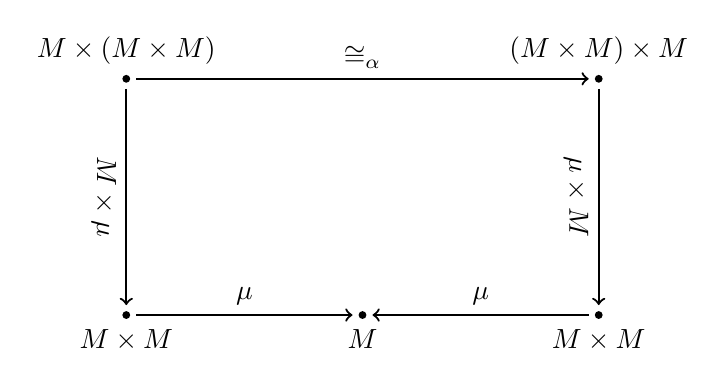
\begin{tikzpicture}[ele/.style={fill=black,circle,minimum
        width=.8pt,inner sep=1pt},every fit/.style={ellipse,draw,inner
        sep=-2pt}]

    % the texts
    
    \node[ele,label=above:$M\times\left(M \times M\right)$] (M31) at (0,3) {};    
    \node[ele,label=above:$\left(M \times M\right)\times M$] (M32) at (6,3) {};    
    \node[ele,label=below:$M \times M$] (M21) at (0,0) {};    
    \node[ele,label=below:$M \times M$] (M22) at (6,0) {};    
    \node[ele,label=below:$M$] (M) at (3,0) {};    

    \draw[->,thick,shorten <=2pt,shorten >=2pt] (M31) to
    node[sloped,above]{$\cong_\alpha$} (M32);
    \draw[->,thick,shorten <=2pt,shorten >=2pt] (M31) to
    node[sloped,below]{$\idm{M} \times \mu$} (M21);
    \draw[->,thick,shorten <=2pt,shorten >=2pt] (M32) to
    node[sloped,below]{$\mu \times \idm{M}$} (M22);
    \draw[->,thick,shorten <=2pt,shorten >=2pt] (M22) to
    node[sloped,above]{$\mu$} (M);
    \draw[->,thick,shorten <=2pt,shorten >=2pt] (M21) to
    node[sloped,above]{$\mu$} (M);
  \end{tikzpicture}
  \caption{Commutative diagram for $\mu\circ\left[\mu \times
    \idm{M}\right] = \mu \circ \left[\idm{M} \times \mu\right] \circ
    \alpha$.} 
  \label{fig:monoid_mu_alpha}
\end{figure}
Very often the isomorphism $\alpha$ is omitted i.e. 
\[
M\times\left(M \times M\right)
= \left(M \times M\right)\times M = M^3
\]
and the morphism
equality \eqref{eq:monad_monoid_mu} is written as follow
\[
\mu\circ\left[\mu \times \idm{M}\right] =
\mu \circ \left[\idm{M} \times \mu\right].
\]
The corresponding commutative diagram is shown in
\cref{fig:monoid_mu}.
\begin{figure}
  \centering
  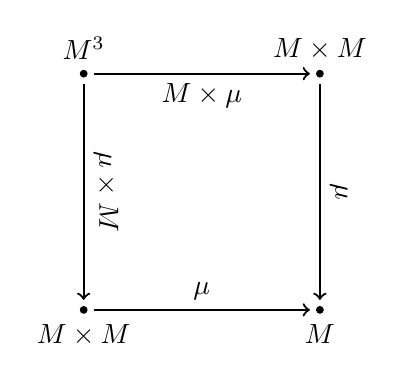
\begin{tikzpicture}[ele/.style={fill=black,circle,minimum
        width=.8pt,inner sep=1pt},every fit/.style={ellipse,draw,inner
        sep=-2pt}]

    % the texts
    
    \node[ele,label=above:$M^3$] (M3) at (0,3) {};    
    \node[ele,label=above:$M \times M$] (M21) at (3,3) {};    
    \node[ele,label=below:$M \times M$] (M22) at (0,0) {};    
    \node[ele,label=below:$M$] (M) at (3,0) {};    

    \draw[->,thick,shorten <=2pt,shorten >=2pt] (M3) to
    node[sloped,below]{$\idm{M} \times \mu$} (M21);
    \draw[->,thick,shorten <=2pt,shorten >=2pt] (M3) to
    node[sloped,above]{$\mu \times \idm{M}$} (M22);
    \draw[->,thick,shorten <=2pt,shorten >=2pt] (M22) to
    node[sloped,above]{$\mu$} (M);
    \draw[->,thick,shorten <=2pt,shorten >=2pt] (M21) to
    node[sloped,above]{$\mu$} (M);
  \end{tikzpicture}
  \caption{Commutative diagram for $\mu\circ\left[\mu \times
    \idm{M}\right] = \mu \circ \left[\idm{M} \times \mu\right]$}
  \label{fig:monoid_mu}
\end{figure}

\subsection{Identity presence}
For \eqref{eq:monoid2} consider a morphism $\eta$ from
\mynameref{def:singleton_set} 
\footnote{
 It also is called \cite{bib:maclane98} as a one point set
}
$I = \{0\}$ to the special element $e \in M$ such that
$\forall m \in M: e \cdot m = m \cdot e = m$. I.e. $\eta: I \to M$ and
$e = \eta(0)$. Consider 2 sets $B = I \times M$ and $B' = M \times I$. 
We have 2 \mynameref{def:isomorphism}s: $B \cong_\lambda M$ and $B'
\cong_\rho M$ such that
\[
\lambda(m) = 0 \times m
\] 
and
\[
\rho(m) = m \times 0.
\] 

If we apply the products (see \mynameref{def:product_of_morphisms}) $\eta \times \idm{M}$ and
$\idm{M} \times \eta$ on $B$ and $B'$ respectively then we get
\begin{eqnarray}
\left[\eta \times \idm{M} \right]\left(0 \times m\right) = e \times m,
\nonumber \\
\left[\idm{M} \times \eta \right]\left(m \times 0\right) = m \times e.
\nonumber
\end{eqnarray}
After the application of $\mu$ on the result we obtain
\begin{eqnarray}
\mu \left(\left[\eta \times \idm{M}\right] \left(0 \times m\right) \right) 
= \mu \left( e \times m \right) = e \cdot m,
\nonumber \\
\mu \left(\left[ \idm{M} \times \eta \right]\left(m \times 0\right) \right) = 
\mu \left(m \times e \right) = m \cdot e.
\nonumber
\end{eqnarray}
\begin{figure}
  \centering
  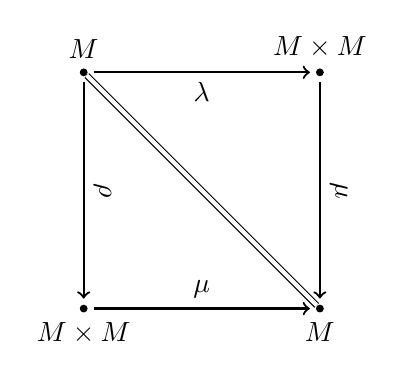
\begin{tikzpicture}[ele/.style={fill=black,circle,minimum
        width=.8pt,inner sep=1pt},every fit/.style={ellipse,draw,inner
        sep=-2pt}]

    % the texts
    
    \node[ele,label=above:$M$] (M') at (0,3) {};    
    \node[ele,label=above:$M \times M$] (M21) at (3,3) {};    
    \node[ele,label=below:$M \times M$] (M22) at (0,0) {};    
    \node[ele,label=below:$M$] (M) at (3,0) {};    

    \draw [double equal sign distance] (M') to (M);
    \draw[->,thick,shorten <=2pt,shorten >=2pt] (M') to
    node[sloped,below]{$\lambda$} (M21);
    \draw[->,thick,shorten <=2pt,shorten >=2pt] (M') to
    node[sloped,above]{$\rho$} (M22);
    \draw[->,thick,shorten <=2pt,shorten >=2pt] (M22) to
    node[sloped,above]{$\mu$} (M);
    \draw[->,thick,shorten <=2pt,shorten >=2pt] (M21) to
    node[sloped,above]{$\mu$} (M);
  \end{tikzpicture}
  \caption{Commutative diagram for $\mu \circ (\eta \times \idm{M})
    \circ \lambda = \mu \circ (\idm{M} \times \mu) \circ \rho =
    \idm{M}$ .} 
  \label{fig:monoid_eta_lambda_rho}
\end{figure}
The \eqref{eq:monoid2} leads to the following equation for morphisms
\[
\mu \circ (\eta \times \idm{M}) \circ \rho = 
\mu \circ (\idm{M} \times \mu) \circ \lambda = 
\idm{M}
\]
or the commutative diagram shown on \cref{fig:monoid_eta_lambda_rho}.

\subsection{Categorical definition for monoid}
Before given a formal definition lets look at the operations were used
for the construction. The first one is the product of 2 objects:
\[
M \times M.
\]
We also have 2 pairs of morphisms:
\begin{eqnarray}
\mu: M \times M \to M,
\nonumber \\
\idm{M}: M \to M.
\nonumber
\end{eqnarray}
and
\begin{eqnarray}
\eta: I \to M, 
\nonumber \\
\idm{M}: M \to M.
\nonumber
\end{eqnarray}
The pairs can be combined into one using
\mynameref{def:product_of_morphisms} as follows:
\begin{eqnarray}
\mu \times \idm{M}: \left(M \times M\right) \times M \to M \times M,
\nonumber \\
\idm{M} \times \mu: M \times \left(M \times M\right) \to M \times M
\nonumber
\end{eqnarray}
and
\begin{eqnarray}
\eta \times \idm{M}: I \times M \to M \times M,
\nonumber \\
\idm{M} \times \eta: M \times I \to M \times M.
\nonumber
\end{eqnarray}
The same structure 
\footnote{not only objects mapping but also morphisms mapping}
is used by
\mynameref{def:functor} 
and
especially by \mynameref{ex:product_bifunctor}.  

%% If we take into consideration that one-point set is
%% \mynameref{ex:set_terminal_object} then we can conclude that the
%% monoid can be defined for instance in a \mynameref{def:cartesian_closed_category}
%% as follow
Now we are ready to provide the monoid definition in the terms of morphisms.
\begin{definition}[Monoid]
\label{def:monoid_category}
Consider \mynameref{def:setcategory} $\cat{C}$ with a
\mynameref{def:singleton_set} $t \in \catob{C}$. The \mynameref{def:cartesian_product}
with \mynameref{def:product_of_morphisms} forms a
\mynameref{def:bifunctor} $\times$ (see \cref{ex:product_bifunctor}).
The object $m \in
\catob{C}$ is called \textit{monoid} if the following
conditions satisfied:
\begin{enumerate}
\item there is a \mynameref{def:morphism} $\mu: m \times m \to m$ in
  the category
\item there is another morphism $\eta: t \to m$ in the category
\item the morphisms satisfy the following conditions:
\begin{equation}
\mu\circ\left(\mu \times
    \idm{M}\right) = \mu \circ \left(\idm{M} \times \mu\right) \circ
    \alpha,
\label{eq:monoid_def_mu}
\end{equation}
\begin{equation}
\mu \circ (\eta \times \idm{M})
\circ \lambda = \mu \circ (\idm{M} \times \mu) \circ \rho =
\idm{M}
\label{eq:monoid_def_eta}
\end{equation}
where $\alpha$ (associator) is an \mynameref{def:isomorphism} between
$m \times (m \times m)$ and $(m \times m) \times m$. $\lambda, \rho$
are other isomorphisms:  
\[
m \cong_\lambda t \times m
\]
and
\[
m \cong_\rho m \times t 
\]
\end{enumerate}
\end{definition}

\section{Monoidal category}
As we saw in the categorical definition for monoid (see
\cref{def:monoid_category}) the category $\cat{C}$ should satisfy
several conditions to have an object as monoid. Lets formalise the conditions.
\begin{definition}[Monoidal category]
\label{def:monoidal_category}
A category $\cat{C}$ is called \textit{monoidal category} if it is
equipped with a \mynameref{def:monoid} structure i.e. there are
\begin{itemize}
\item \mynameref{def:bifunctor} $\otimes: \cat{C} \times \cat{C} \tof
  \cat{C}$ called \textit{monoidal product} \index{Monoidal
    product!definition} 
\item an \mynameref{def:object} $e$ called unit object or identity object
\end{itemize}

The elements should satisfy (up to \mynameref{def:isomorphism})
several conditions. The first one:
associativity: 
\begin{equation}
a \otimes \left( b \otimes c \right) \cong_\alpha
  \left( a \otimes b \right) \otimes c,
\nonumber
\end{equation}
where $\alpha$ is called associator. \index{Associator!definition}
The second condition says that
$e$ can be treated as left and right identity: 
\begin{eqnarray}
a \cong_\lambda e \otimes a, 
\nonumber \\
a \cong_\rho a \otimes e,
\nonumber
\end{eqnarray}
where $\lambda, \rho$ are called as left and right unitors respectively. \index{Left unitor!definition} \index{Right unitor!definition}
\end{definition}

In the \mynameref{def:setcategory} we have $\times$ as the monoidal
product (see \cref{ex:product_bifunctor}). There is also a
morphism $\eta$ from terminal object $t$ to $e$
\cite{bib:stackexchange:terminalinmonoid} (see \cref{def:monoid_category}). 

\begin{definition}[Strict monoidal category]
\label{def:strict_monoidal_category}
\index{Associator}
A \mynameref{def:monoidal_category} $\cat{C}$ is said to be \textit{strict} if the
associator, left and right unitors are all identity morphisms i.e.
\[
\alpha = \lambda = \rho = \idm{C}.
\]
\index{Left unitor} \index{Right unitor}
\end{definition}

\begin{remark}[Monoidal product]
\label{rem:monoidal_product}
The monoidal product is a binary operation that specifies the exact
monoidal structure. Often it is called as \textit{tensor product} but
we will avoid the naming because it is not always the same as the
\mynameref{def:tensor_product} introduced for
\mynameref{def:hilbert_space}s. We also note that the monoidal product is
a \mynameref{def:bifunctor}. 
\end{remark}

\section{Tensor product in Quantum mechanics}

\begin{definition}[Tensor product]
  \label{def:tensor_product}
  Let $m,n \in \cat{FdHilb}$. The \textit{tensor product} $m \otimes n$ is another
  finite dimensional \mynameref{def:hilbert_space} equipped with a
  bilinear form
  \[
  \phi: m \times n \to m \otimes n
  \]
  such that $\forall a \in \cat{FdHilb}$ and for any
  bilinear
  \[
  f: m \times n \to a
  \]
  exists only one morphism $\tilde{f}: m \times n \to a$ such that
  \[
  f = \tilde{f} \circ \phi
  \]
  i.e. the diagram on the \cref{fig:tensor_product} commutes
\begin{figure}[H]
  \centering
  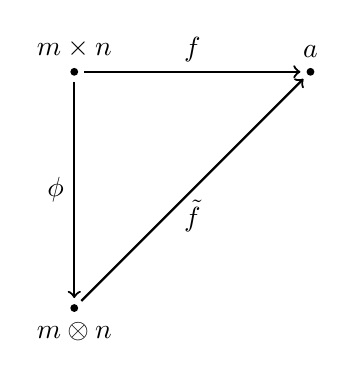
\begin{tikzpicture}[ele/.style={fill=black,circle,minimum
        width=.8pt,inner sep=1pt},every fit/.style={ellipse,draw,inner
        sep=-2pt}]

    % the texts
    
    \node[ele,label=above:$m \times n$] (mn) at (0,3) {};    
    \node[ele,label=above:$a$] (a) at (3,3) {};    
    \node[ele,label=below:$m \otimes n$] (mxn) at (0,0) {};    

    \draw[->,thick,shorten <=2pt,shorten >=2pt] (mn) to
    node[above]{$f$} (a);
    \draw[->,thick,shorten <=2pt,shorten >=2pt] (mn) to
    node[left]{$\phi$} (mxn);
    \draw[->,thick,shorten <=2pt,shorten >=2pt] (mxn) to
    node[below]{$\tilde{f}$} (a);
  \end{tikzpicture}
  \caption{Commutative diagram for tensor product definition.} 
  \label{fig:tensor_product}
\end{figure}
\end{definition}

\begin{remark}[Tensor product]
Using the fact that \mynameref{def:linear_map}s are
\mynameref{def:morphism}s in $\cat{FdHilb}$ we can conclude that 
\mynameref{def:tensor_product} is a \mynameref{def:bifunctor}.
\end{remark}

The tensor product in quantum mechanics is used for
representing a system that consists of multiple systems. For instance
if we have an interaction between an 2 level atom ($a$ is excited
state $b$ as a ground state) and one mode light then the
atom has its own Hilber space $\mathcal{H}_{at}$ with $\ket{a}$ and
$\ket{b}$ as basis 
vectors.  Light also has its own Hilber space $\mathcal{H}_f$ with Fock state
$\{\ket{n}\}$ as the basis.
\footnote{
  Really the $\mathcal{H}_f$ is infinite dimensional Hilber space and
  seems to be out of our assumption about $\cat{FdHilb}$ category as
  a collection of finite dimensional Hilber spaces only.
}
The result system that describes both atom
and light is represented as the tensor product $\mathcal{H}_{at}
\otimes \mathcal{H}_f$.

\begin{remark}[Hilbert-Schmidt correspondence]
The morphisms of $\cat{FdHilb}$ category have a connection with
\mynameref{def:tensor_product}. Consider the so called Hilbert-Schmidt
correspondence for finite dimensional Hilbert spaces i.e. for given
$\mathcal{A}$ and $\mathcal{B}$ there is a natural isomorphism between
the tensor product and \mynameref{def:linear_map}s (aka morphisms) between
$\mathcal{A}$ and $\mathcal{B}$:
\[
\mathcal{A}^\ast \otimes \mathcal{B} \cong \hom(\mathcal{A}, \mathcal{B})
\]
where $\mathcal{A}^\ast$ - \mynameref{def:dual_space}.
\end{remark}

\section{Category of endofunctors}

The \mynameref{def:funcategory} is an example of a category. We can
apply additional limitation and consider only
\mynameref{def:endofunctor}s i.e. we will look at the category
$[\cat{C}, \cat{C}]$ - the category of functors from category $\cat{C}$ to
the same category. One of the most popular math definition of a monad
is the following: 
``All told, a monad in X is just a monoid in the category of
endofunctors of X''\cite{bib:maclane98}.
Later we will give an explanation for that one.

We start with the formal definition of category of endofunctors and a
tensor product in the category
\begin{definition}[Category of endofunctors]
\label{def:category_of_endofunctors}
Let $\cat{C}$ is a category, then  the category $[\cat{C}, \cat{C}]$ of
functors from category $\cat{C}$ to the same category is called the
category of endofunctors. The monoidal product in the category is the
functor composition. 
\end{definition}

\begin{definition}[Monad]
  \label{def:monad}
  The monad $M$ is an \mynameref{def:endofunctor} with 2
  \mynameref{def:nt}s:
  \begin{equation}
    \label{eq:monad_mu}
    \mu: M \circ M \tont M
  \end{equation}
  and
  \begin{equation}
    \label{eq:monad_eta}
    \eta: \idf{C} \tont M,
  \end{equation}
  where $\idf{C}$ is \mynameref{def:idfunctor}.

  The $\eta, \mu$ should satisfy the following conditions:
  \begin{eqnarray}
    \mu \circ M \mu = \mu \circ \mu M, 
    \nonumber \\
    \mu \circ M \eta = \mu \circ \eta M = \idnt{M},
    \label{eq:monad}
  \end{eqnarray}
  where $M \mu, M \eta$ - \mynameref{def:rw}s, $\mu M, \eta M$ -
  \mynameref{def:lw}s, $\idnt{M}$ - \mynameref{def:idnt} for $M$.
  \mynameref{def:vertical_composition} is used in the equations.

  The monad will be denoted later as $\left<M, \mu, \eta\right>$.
\end{definition}

Lets look at the requirements \eqref{eq:monad} more closely. Notice
that the functor composition is associative:
\[
M \circ ( M \circ M ) = (M \circ M) \circ M = M^3.
\]
Secondly 
all rewrite it with \eqref{eq:lw} and \eqref{eq:rw} as follows
\begin{eqnarray}
  \mu \circ \left( \idnt{M} \star \mu \right) = 
  \mu \circ \left( \mu \star \idnt{M} \right), 
  \nonumber \\
  \mu \circ \left( \idnt{M} \star \eta \right) = 
  \mu \circ \left( \eta \star \idnt{M} \right) = \idnt{M}.
  \label{eq:monad_p1}
\end{eqnarray}
Thus we can notice that the pair of operations (composition $\circ$
and \mynameref{def:horizontal_composition} $\star$) forms the bifunctor (see
\mynameref{rem:bifunctor_fun_cat}). 

The morphism $\idnt{M} \star \mu$ acts on $M \circ ( M \circ M )$ as
\[
\idnt{M} \star \mu : M \circ ( M \circ M ) \tont M \circ (M \otimes M)
\]
thus
\[
\mu \circ (\idnt{M} \star \mu) : M \circ ( M \circ M ) \tont M \otimes (M \otimes M).
\]
Similarly 
\[
\mu \circ (\mu \star \idnt{M}) : (M \circ  M) \circ M  \tont ( M \otimes M) \otimes M.
\]
I.e. the both morphisms start at the same object $M^3$ and finish also
at the same point. The equality 
\begin{equation}
\mu \circ (\idnt{M} \star \mu) = 
\mu \circ (\mu \star \idnt{M})
\label{eq:monoidalobject1}
\end{equation}
is similar to the conditions on the \cref{fig:monoid_mu} and can be
written as \cref{fig:monad_monoid1}. Thus if we compare
\eqref{eq:monoidalobject1} and \eqref{eq:monoid_def_mu} then we can say
that they are same if we replace $\star$ sign with $\times$ one. I.e.
in the case we can say that the monad looks like a
\mynameref{def:monoid_category}. 

\begin{figure}
  \centering
  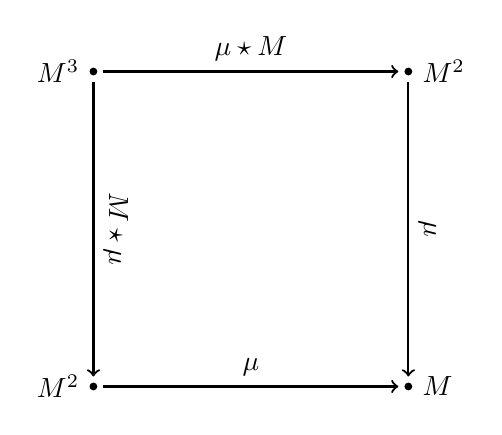
\begin{tikzpicture}[ele/.style={fill=black,circle,minimum
        width=.8pt,inner sep=1pt},every fit/.style={ellipse,draw,inner
        sep=-2pt}]

    % the texts
    
    \node[ele,label=left:$M^3$] (m3) at (0,4) {};    
    \node[ele,label=left:$M^2$] (m21) at (0,0) {};    
    \node[ele,label=right:$M^2$] (m22) at (4,4) {};
    \node[ele,label=right:$M$] (m) at (4,0) {};

    \draw[->,thick,shorten <=2pt,shorten >=2pt] (m3) to
    node[sloped,above]{$\idnt{M} \star \mu$} (m21);
    \draw[->,thick,shorten <=2pt,shorten >=2] (m3) to
    node[sloped,above]{$\mu \star \idnt{M}$} (m22); 
    \draw[->,thick,shorten <=2pt,shorten >=2] (m21) to
    node[sloped,above]{$\mu$} (m); 
    \draw[->,thick,shorten <=2pt,shorten >=2] (m22) to
    node[sloped,above]{$\mu$} (m); 
  \end{tikzpicture}
  \caption{Monad as monoid in the category of endofunctors.}
  \label{fig:monad_monoid1}
\end{figure}

For the identity element consider the same trick: replace in
\eqref{eq:monoid_def_eta} tensor
product $\times$ with \mynameref{def:horizontal_composition} $\star$ and
morphisms $\idm{M}, \rho, \lambda$ with identity natural transformation
$\idnt{M}$. Thus the equation
\[
\mu \circ (\eta \times \idm{M})
\circ \lambda = \mu \circ (\idm{M} \times \mu) \circ \rho =
\idm{M}
\]
will be replaced with
\[
\mu \circ (\eta \star \idnt{M}) = \mu \circ (\idnt{M} \star \mu) =
\idnt{M}
\]
that is the exact we want to get (see second equation of
\eqref{eq:monad_p1}). 

%% There should be an identity element for each \mynameref{def:monoid}.
%% Lets show that the second equation of  \eqref{eq:monad_p1} provides us
%% the required element. Lets $U =
%% \eta\left(\idf{C}\right)$. 
%% We want to show that 
%% \begin{equation}
%% U \otimes M = M \otimes U = M, 
%% \nonumber
%% \end{equation}
%% that is exactly required as identity presence in the
%% \mynameref{def:monoid} definition.
%% Consider the action of the left part of second equation
%% \eqref{eq:monad_p1} on $M = M \circ \idf{C}$:
%% \begin{eqnarray}
%% \mu \circ \left( \idnt{M} \star \eta \right) \left[M \circ \idf{C}\right] = 
%% \nonumber \\
%% =
%% \mu \left[M \circ U\right] = M \otimes U
%% \nonumber
%% \end{eqnarray}
%% For the middle part of  of second equation
%% \eqref{eq:monad_p1}
%% \begin{eqnarray}
%% \mu \circ \left( \eta \star \idnt{M} \right) \left[M\right] = 
%% \mu \circ \left( \eta \star \idnt{M} \right) \left[\idf{C} \circ M\right] = 
%% \nonumber \\
%% =
%% \mu \left[U \circ M\right] = U \otimes M.
%% \nonumber
%% \end{eqnarray}
%% Thus
%% finally
%% \[
%% M \otimes U = U \otimes M = M
%% \]
%% that finals the proof of monoidal structure.

\section{Monads in programming languages}
There are several examples of \mynameref{def:monad} implementation in
different programming languages:

\subsection{Haskell}

\begin{example}[Monad][$\cat{Hask}$]
\label{ex:monad_haskell}
In Haskell monad can be defined from \mynameref{ex:functor_haskell} as follows 
\footnote{real definition is quite different from the presented one}
\begin{minted}{haskell}
    class Functor m => Monad m where
        return :: a -> m a
        (>>=)  :: m a -> (a -> m b) -> m b
\end{minted} 

To show how this one can be get we can start from a definition that is
similar to the math definition:
\begin{minted}{haskell}
    class Functor m => Monad m where
        return :: a -> m a
        join  :: m (m a) -> m a
\end{minted} 
where \textbf{return} can be treated as $\eta$
\eqref{eq:monad_eta} and 
\textbf{join} as $\mu$ \eqref{eq:monad_mu}. In the case
the bind operator \textbf{>>=} can be implemented as follows
\begin{minted}{haskell}
(>>=)  :: m a -> (a -> m b) -> m b
ma >>= f = join ( fmap f ma )
\end{minted} 

\end{example}

\subsection{C++}
The monad in C++ use the functor definition from \mynameref{ex:functor_cpp}
\begin{minted}{c++}
// from functor.h
template < template< class ...> class M, class A, class B> 
M<B> fmap(std::function<B(A)>, M<A>);

// file: monad.h
template < template< class ...> class M, class A> 
M<A> pure(A);

template < template< class ...> class M, class A> 
M<A> join(M< M<A> >);
\end{minted}
where \textbf{pure} can be treated as $\eta$
\eqref{eq:monad_eta} and 
\textbf{join} as $\mu$ \eqref{eq:monad_mu}. In the case
the bind operator can be implemented as follows
\begin{minted}{c++}
template < template< class ...> class M, class A, class B> 
M<B> bind(std::function< M<B> (A) > f, M<A> a) {
  return join( fmap<>(f, a) );
};
\end{minted}

\subsection{Scala}

\begin{example}[Monad][$\cat{Scala}$]
The monad concept is Scala is more close to formal math definition for
\mynameref{def:monad}. It can be defined as follows 
\footnote{real definition is quite different from the presented one}
\label{ex:monad_scala}
\begin{minted}{scala}
trait M[A] {
  def flatMap[B](f: A => M[B]): M[B]
}
  
def unit[A](x: A): M[A]
\end{minted} 
I.e. \textbf{flatMap} can be considered as $\mu$ and
\textbf{unit} as $\eta$. 
\end{example}

TBD

